% Chuong 4  --  phu trach: Hùng (xem report/PHANCONG.md)
% Moi muc la mot file s*.tex trong thu muc nay, de nhieu nguoi sua song song khong dung nhau.
% Hinh: sinh boi report/figures/src/make_ch04_serminal.py cua repo 1DCNN (doc results/, export/ cua repo do).
\chapter{Mô hình CNN và pipeline phần mềm}\label{ch:cnn}

Chương này trình bày phần mô hình của hệ thống: dữ liệu và cách đánh giá, khối tiền xử lý tín hiệu, trích xuất đặc trưng, kiến trúc mạng CNN Lite, quá trình huấn luyện và lựa chọn cấu hình, lượng tử hoá int8 và bộ dữ liệu chuẩn dùng để kiểm chứng phần cứng.
Với mỗi khối, chương nêu lựa chọn thiết kế, lý do của lựa chọn đó và kết quả kiểm chứng tương ứng.
Đầu ra của chương là một pipeline đã đóng băng, chỉ dùng phép toán số nguyên, làm chuẩn tham chiếu cho bộ tăng tốc ở Chương~\ref{ch:phancung}.
Kết quả đánh giá cuối cùng trên tập kiểm tra được trình bày riêng ở Mục~\ref{sec:dochinhxac}.

% Muc 4.1  --  phu trach: xem report/PHANCONG.md
\section{Dữ liệu và giao thức đánh giá}\label{sec:dulieu}
\begin{goiy}
  \begin{itemize}
    \item MIT-BIH: 48 bản ghi; loại 102, 104, 107, 217 (paced); chia DS1/DS2 (de Chazal); nhịp trong đoạn VF không tính.
    \item Ánh xạ nhãn AAMI; số nhịp mỗi lớp mỗi tập (Bảng~\ref{tab:dulieu}); lớp Q bị loại.
    \item Huấn luyện: 5-fold nhóm theo bản ghi trên DS1, inner-val 20\,\% cuối theo thời gian; DS2 khoá bằng \texttt{ECG\_ALLOW\_DS2}, chạy một lần.
    \item Chỉ số: macro-F1; Se và $+P$ của SVEB, VEB; Se/$+P$ phát hiện R (dung sai $\pm150$~ms).
  \end{itemize}
\end{goiy}
\bangcho{số bản ghi, số nhịp theo lớp N/S/V/F cho DS1 và DS2}{Thống kê tập dữ liệu và cách chia.}{tab:dulieu}

% Muc 4.2  --  phu trach: Hùng
% nguon: docs/system_overview.md §7 (tang 1-8); python/dsp/pan_tompkins.py (docstring: chuyen 200 -> 360 Hz, nguong);
%        python/quant/pipeline_int.py (loc, tinh chinh R, cua so, z-score, RR so nguyen); python/dsp/filters.py (Butterworth);
%        NHATKY.md cua repo 1DCNN (Se/+P detector DS1); trung vi dac trung RR: cache beats_annotation, 22 ban ghi DS1
\section{Tiền xử lý tín hiệu bằng số nguyên}\label{sec:tienxuly}

Khối tiền xử lý nhận tín hiệu MIT-BIH và cho ra tín hiệu đã lọc $y$ cùng vị trí đỉnh R của từng nhịp, là đầu vào của khối trích xuất đặc trưng ở Mục~\ref{sec:dactrung}.
Mọi bộ lọc đều nhân quả để hệ thống xử lý được tín hiệu theo thời gian thực, và mọi phép tính là số nguyên để phần cứng cài đặt lại vẫn khớp từng bit với mô hình tham chiếu.
Huấn luyện và triển khai dùng chung khối này.

Hình~\ref{fig:tienxuly} trình bày các khối xử lý chính: dữ liệu MIT-BIH đi qua tiền xử lý, trích xuất đặc trưng, mô hình CNN, lượng tử hoá, đánh giá và cuối cùng là xuất dữ liệu; mô hình được trình bày ở Mục~\ref{sec:cnnlite} và Mục~\ref{sec:huanluyen}, lượng tử hoá ở Mục~\ref{sec:luongtu}.
Khối tiền xử lý gồm hai nhánh song song.
Nhánh phát hiện chỉ cần biết nhịp nằm ở đâu, nên được phép làm biến dạng tín hiệu để mỗi phức bộ QRS thành một đỉnh nổi bật.
Nhánh hình dạng phải giữ hình dạng thật của nhịp cho mạng phân loại, nên chỉ lọc nhẹ.
Hình~\ref{fig:ch4-khoitienxuly} bóc tách khối tiền xử lý thành các khâu, và Bảng~\ref{tab:ch4-tienxuly} tóm tắt phép toán và độ trễ của từng khâu.

\begin{figure}[htbp]
  \centering
  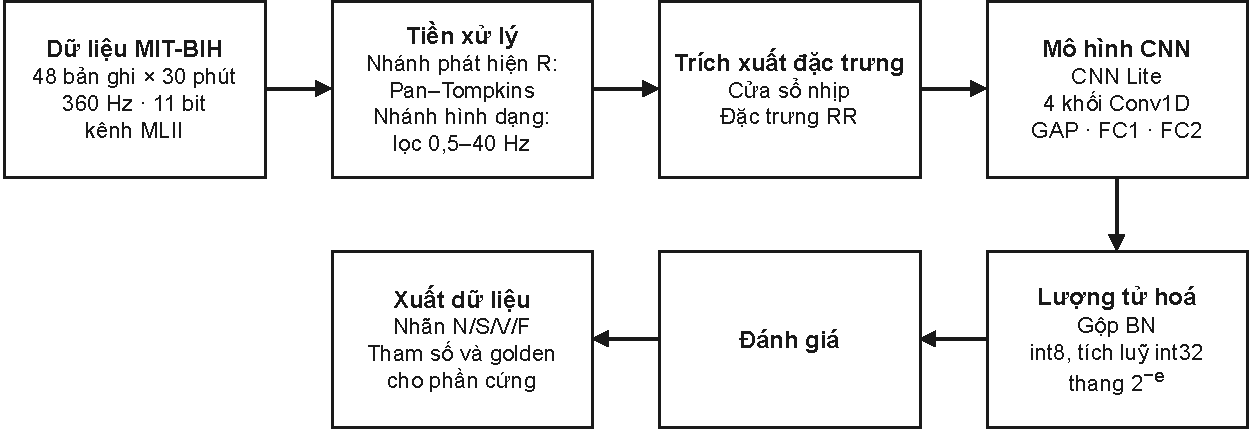
\includegraphics[width=\textwidth]{ch04_mo_hinh_cnn/luong_tong}
  \caption{Các khối xử lý chính của phần mô hình, từ dữ liệu MIT-BIH đến dữ liệu xuất ra.}\label{fig:tienxuly}
\end{figure}

\begin{figure}[htbp]
  \centering
  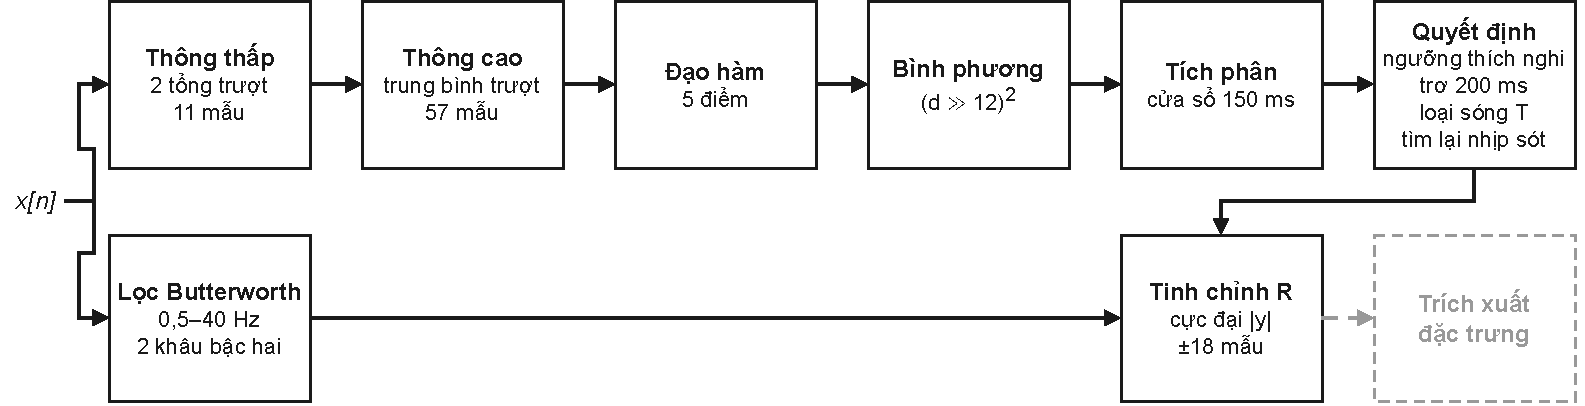
\includegraphics[width=\textwidth]{ch04_mo_hinh_cnn/khoi_tienxuly}
  \caption{Các khâu của khối tiền xử lý: nhánh phát hiện R (hàng trên) và nhánh hình dạng (hàng dưới); khối nét đứt là khối kế tiếp.}\label{fig:ch4-khoitienxuly}
\end{figure}

\begin{table}[htbp]
  \centering
  \caption{Tóm tắt các khâu tiền xử lý số nguyên.}\label{tab:ch4-tienxuly}
  \small\setlength{\tabcolsep}{4pt}
  \begin{tabular}{@{}llll@{}}
    \toprule
    Khâu & Phép toán chính & Đầu ra & Độ trễ \\
    \midrule
    \multicolumn{4}{@{}l}{\emph{Nhánh phát hiện}} \\
    Thông thấp + thông cao & tổng trượt 11, 11 và 57 mẫu & tín hiệu dải 5--12\,Hz & 38 mẫu \\
    Đạo hàm, bình phương & sai phân 5 điểm, dịch 12 bit, nhân & năng lượng sườn dốc & 2 mẫu \\
    Tích phân cửa sổ & tổng trượt 54 mẫu & một đỉnh cho mỗi QRS & 26{,}5 mẫu \\
    Quyết định & ngưỡng thích nghi, dịch bit & vị trí R thô & 0{,}21--0{,}32\,s \\
    \midrule
    \multicolumn{4}{@{}l}{\emph{Nhánh hình dạng}} \\
    Lọc 0{,}5--40\,Hz & 2 khâu bậc hai, hệ số $2^{20}$ & tín hiệu đã lọc & 2 mẫu \\
    Tinh chỉnh R & tìm cực đại trong $\pm18$ mẫu & vị trí R & 0 \\
    \bottomrule
  \end{tabular}
\end{table}

\subsection{Nhánh phát hiện}

Mỗi bản ghi MIT-BIH lưu sẵn các mẫu số nguyên $u[n]$ 11 bit, điểm không ở 1024, 200 đơn vị trên mỗi mV.
Trước hết tín hiệu được đưa về dao động quanh 0:
\begin{equation}
  x[n]=u[n]-1024,\qquad |x[n]|\le2^{10}.
  \label{eq:ch4-adc}
\end{equation}
Biết trước $|x|\le2^{10}$ nên tính được giá trị lớn nhất ở mỗi khâu sau và kiểm được rằng không khâu nào tràn số nguyên 32 bit.

Nhánh phát hiện dùng thuật toán Pan--Tompkins~\cite{pantompkins1985realtime}.
Bản gốc thiết kế cho 200\,Hz; ở 360\,Hz, mọi độ dài và khoảng thời gian được nhân $1{,}8$ rồi làm tròn.
Các phép chia chuẩn hoá của bản gốc được bỏ đi, vì chúng chỉ đổi thang tín hiệu còn các ngưỡng phía sau tự thích nghi theo biên độ.
Năm khâu của nhánh là:
\begin{align}
  \mathrm{lp}[n]&=\sum_{k=0}^{10}s[n-k],\quad s[n]=\sum_{k=0}^{10}x[n-k], \label{eq:ch4-lp}\\
  \mathrm{hp}[n]&=57\cdot\mathrm{lp}[n-28]-\sum_{k=0}^{56}\mathrm{lp}[n-k], \label{eq:ch4-hp}\\
  d[n]&=2\,\mathrm{hp}[n]+\mathrm{hp}[n-1]-\mathrm{hp}[n-3]-2\,\mathrm{hp}[n-4], \label{eq:ch4-der}\\
  q[n]&=\big(d[n]\gg12\big)^{2}, \label{eq:ch4-sq}\\
  \mathrm{mwi}[n]&=\sum_{k=0}^{53}q[n-k]. \label{eq:ch4-mwi}
\end{align}
\begin{itemize}
  \item \textbf{Thông thấp} \eqref{eq:ch4-lp}: hai tổng trượt dài 11 mẫu (bản gốc dài 6) nối tiếp, cho đáp ứng xung hình tam giác và loại nhiễu tần cao.
  \item \textbf{Thông cao} \eqref{eq:ch4-hp}: tín hiệu trễ trừ trung bình trượt của chính nó, chỉ còn lại phần biến đổi nhanh.
  Độ dài 57 (bản gốc 32) là số lẻ để độ trễ 28 mẫu là số nguyên; nhân số hạng trễ với 57 thay cho chia tổng cho 57.
  Hai khâu lọc tạo thành bộ thông dải 4{,}9--11{,}8\,Hz ở mức $-3$\,dB, là dải chứa phần lớn năng lượng QRS, với tổng độ trễ 38 mẫu.
  \item \textbf{Đạo hàm} \eqref{eq:ch4-der}: công thức năm điểm của bản gốc, bỏ hệ số $1/8$, làm nổi bật sườn dốc của QRS so với sóng P và T.
  \item \textbf{Bình phương} \eqref{eq:ch4-sq}: đưa mọi giá trị về dương và khuếch đại sườn dốc; dịch 12 bit trước để kết quả vừa 32 bit.
  \item \textbf{Tích phân} \eqref{eq:ch4-mwi}: cửa sổ 54 mẫu bằng 150\,ms, xấp xỉ độ rộng QRS, gộp mỗi phức bộ thành một đỉnh; giá trị lớn nhất $2^{29{,}3}$ vẫn nhỏ hơn $2^{31}$.
\end{itemize}

Khối quyết định xếp mỗi đỉnh của $\mathrm{mwi}$ vào loại nhịp hoặc nhiễu.
Theo bản gốc, khối giữ mức đỉnh nhịp $\mathrm{SPK}$ và mức đỉnh nhiễu $\mathrm{NPK}$, cập nhật mỗi khi có một đỉnh cao $p$, rồi suy ra hai ngưỡng:
\begin{equation}
  \begin{gathered}
  \mathrm{SPK}\leftarrow\mathrm{SPK}+\big((p-\mathrm{SPK})\gg3\big),\\
  \mathrm{THR1}=\mathrm{NPK}+\big((\mathrm{SPK}-\mathrm{NPK})\gg2\big),\qquad
  \mathrm{THR2}=\mathrm{THR1}\gg1,
  \end{gathered}
  \label{eq:ch4-thr}
\end{equation}
với $\mathrm{NPK}$ cập nhật giống $\mathrm{SPK}$.
Công thức gốc $\mathrm{SPK}\leftarrow0{,}125\,p+0{,}875\,\mathrm{SPK}$ được viết lại thành dịch phải 3 bit, cho kết quả như nhau trên số nguyên mà không cần phép nhân.
$\mathrm{THR1}$ nằm ở một phần tư khoảng từ mức nhiễu lên mức nhịp, nên tự thích ứng khi biên độ thay đổi giữa các bệnh nhân.
Một đỉnh là nhịp khi vượt ngưỡng trên cả $\mathrm{mwi}$ và tín hiệu thông dải.
Khối áp dụng thêm ba quy tắc sinh lý: bỏ qua mọi đỉnh trong 200\,ms sau một nhịp vì cơ tim chưa thể co lại; coi đỉnh trong vòng 360\,ms có độ dốc nhỏ hơn một nửa nhịp trước là sóng T; nếu sau $1{,}66$ lần RR trung bình chưa có nhịp thì tìm lại với ngưỡng $\mathrm{THR2}$, trong đó $1{,}66$ được xấp xỉ bằng $1+\tfrac12+\tfrac18+\tfrac1{32}$.

Hình~\ref{fig:ch4-pt} cho thấy tín hiệu qua các khâu trên một đoạn có nhịp N xen nhịp V.
Sau thông dải chỉ còn dao động quanh QRS; sau tích phân mỗi QRS là một đỉnh rộng, và $\mathrm{THR1}$ nằm dưới đỉnh của cả hai loại nhịp nên không nhịp nào bị bỏ sót.
Trên DS1, bộ phát hiện đạt độ nhạy 99{,}633\,\% và độ chính xác dương 99{,}146\,\%.

\begin{figure}[htbp]
  \centering
  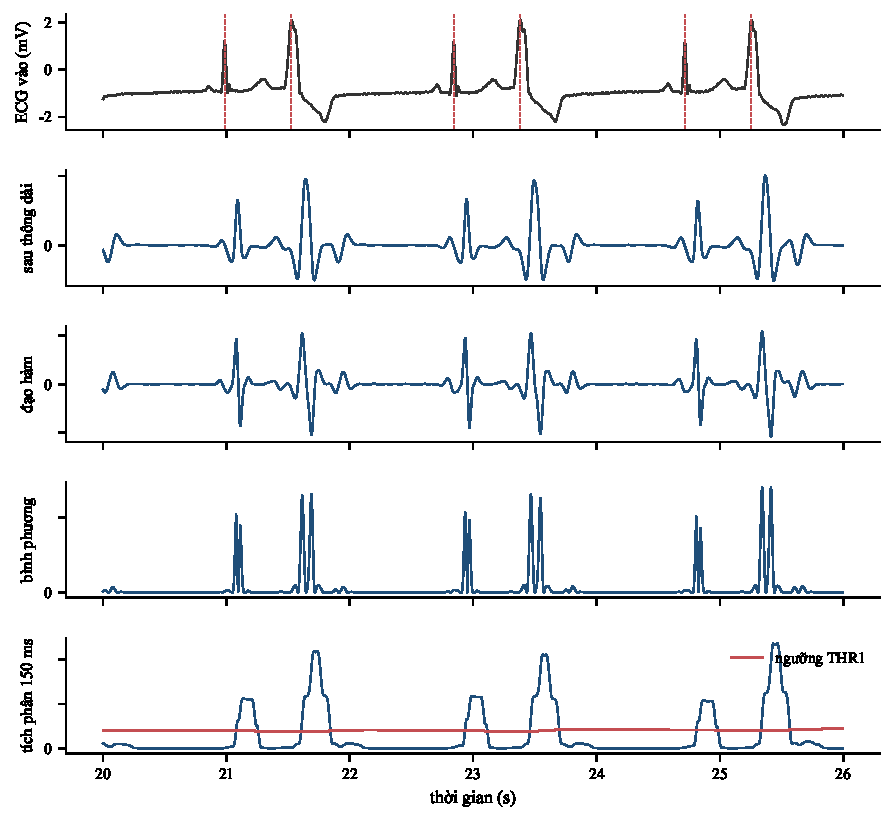
\includegraphics[width=\textwidth]{ch04_mo_hinh_cnn/pt_cackhau.pdf}
  \caption{Tín hiệu qua các khâu Pan--Tompkins số nguyên trên 6\,s của bản ghi 119 (DS1). Đường đứt nét ở hàng trên là vị trí R được phát hiện; đường đỏ ở hàng dưới là ngưỡng thích nghi $\mathrm{THR1}$.}\label{fig:ch4-pt}
\end{figure}

\subsection{Nhánh hình dạng}

\paragraph{Lọc thông dải.}
Bộ lọc Butterworth 0{,}5--40\,Hz loại trôi đường nền do hô hấp, cử động (dưới 0{,}5\,Hz) và nhiễu cơ, nhiễu điện lưới (trên 40\,Hz), nhưng vẫn giữ sóng P, QRS và T.
Butterworth có dải thông phẳng nên không làm méo biên độ tương đối giữa các sóng; bậc thấp cho ít hệ số và ổn định khi làm tròn.
Bộ lọc gồm hai khâu bậc hai nối tiếp, mỗi khâu tính theo
\begin{equation}
  y[n]=b_0x[n]+b_1x[n-1]+b_2x[n-2]-a_1y[n-1]-a_2y[n-2].
  \label{eq:ch4-biquad}
\end{equation}
Khâu thứ nhất có tử số $(1+z^{-1})^2$, triệt tần cao; khâu thứ hai có tử số $(1-z^{-1})^2$, triệt thành phần một chiều.
Trên số nguyên, hệ số được nhân $2^{20}$, tín hiệu được nhân $2^{12}$, tổng tính trên 64 bit rồi đổi thang bằng $y=(\mathrm{acc}+2^{19})\gg20$; sai lệch so với bộ lọc số thực khoảng 0{,}1\,\%.
Hệ số cụ thể ở Phụ lục~\ref{pl:luongtu}.

\paragraph{Tinh chỉnh R.}
Vị trí R thô $r_c$ lấy từ tín hiệu đã biến dạng nên có thể lệch vài mẫu; nó được dời về điểm có biên độ tuyệt đối lớn nhất trong $\pm50$\,ms của tín hiệu đã lọc $y$:
\begin{equation}
  R=\underset{|r-r_c|\le18}{\arg\max}\;\big|y[r+D]\big|,
  \label{eq:ch4-refine}
\end{equation}
với $D=2$ là độ trễ của bộ lọc.
Trị tuyệt đối giúp tìm đúng đỉnh cả khi QRS hướng xuống, như ở nhiều nhịp V.

% Muc 4.3 (moi, tach tu muc 4.2)  --  phu trach: Hùng
% nguon: python/quant/pipeline_int.py (cua so, z-score, RR so nguyen); docs/system_overview.md §7 (tang 6-8);
%        trung vi dac trung RR: cache beats_annotation cua repo 1DCNN, 22 ban ghi DS1
\section{Trích xuất đặc trưng}\label{sec:dactrung}

Từ tín hiệu đã lọc $y$ và vị trí đỉnh R của khối tiền xử lý, khối trích xuất đặc trưng tạo ra hai đầu vào của mạng cho mỗi nhịp: cửa sổ $z_q$ gồm 360 giá trị int8 mô tả hình dạng nhịp và bốn đặc trưng $\mathrm{rr}_q$ mô tả nhịp điệu.
Hình~\ref{fig:ch4-khoidactrung} trình bày hai nhánh của khối.

\begin{figure}[htbp]
  \centering
  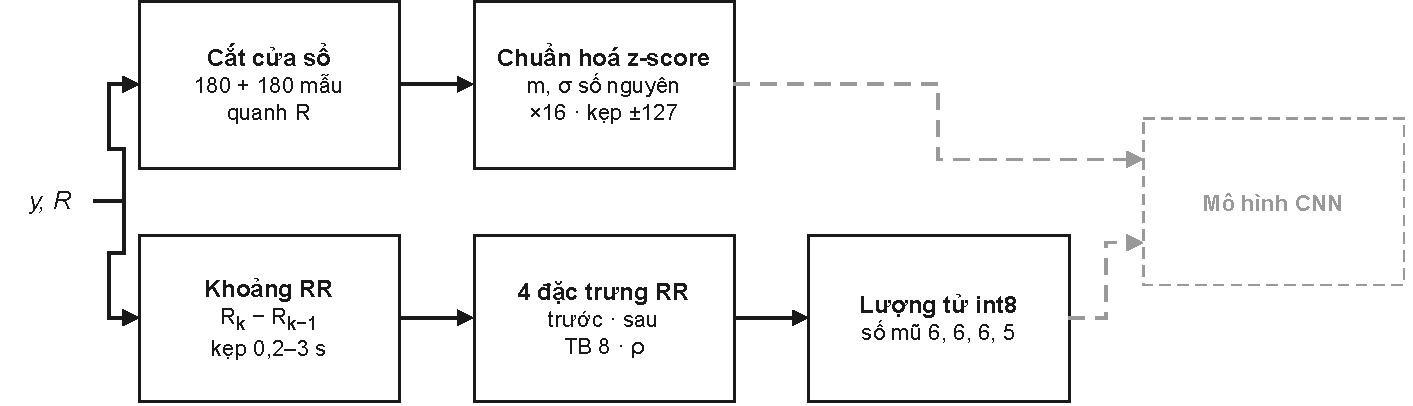
\includegraphics[width=\textwidth]{ch04_mo_hinh_cnn/khoi_dactrung}
  \caption{Các khâu của khối trích xuất đặc trưng: nhánh hình dạng (hàng trên) và nhánh nhịp điệu (hàng dưới); khối nét đứt là khối kế tiếp.}\label{fig:ch4-khoidactrung}
\end{figure}

\subsection{Cửa sổ nhịp và chuẩn hoá z-score}

Mỗi nhịp được biểu diễn bằng 360 mẫu tín hiệu đã lọc quanh đỉnh R:
\begin{equation}
  w_i=y[R+D-180+i],\qquad i=0,\ldots,359,
  \label{eq:ch4-window}
\end{equation}
với $D=2$ là độ trễ của bộ lọc.
Cửa sổ dài 1\,s, đủ bao sóng P và sóng T của nhịp đang xét ở nhịp tim 60--100 nhịp/phút.

Biên độ ECG khác nhau giữa các bệnh nhân và các lần đặt điện cực, nên mỗi cửa sổ được chuẩn hoá theo chính nó, $z=(w-m)/\sigma$, viết bằng số nguyên:
\begin{equation}
  \begin{gathered}
  m=\left\lfloor\frac{1}{360}\sum_{i}w_i\right\rceil,\qquad
  \sigma=\left\lfloor\sqrt{\left\lfloor\frac{1}{360}\sum_{i}(w_i-m)^2\right\rceil}\,\right\rfloor,\\
  z_{q,i}=\mathrm{clamp}\left(\left\lfloor\frac{16\,(w_i-m)}{\sigma+1}\right\rceil,\,-127,\,127\right),
  \end{gathered}
  \label{eq:ch4-zscore}
\end{equation}
với $\lfloor\cdot\rceil$ là chia làm tròn và $\lfloor\sqrt{\cdot}\rfloor$ là căn bậc hai số nguyên.
Hệ số 16 khớp với thang $2^{-4}$ của đầu vào mạng; số hạng $+1$ tránh chia cho 0 và ứng với $\epsilon=10^{-6}$\,mV của bản số thực; phép kẹp $\pm127$ là giới hạn int8, tương ứng khoảng $\pm7{,}9$ độ lệch chuẩn.
Hình~\ref{fig:ch4-motnhip} minh hoạ các bước trên một nhịp V.

\begin{figure}[htbp]
  \centering
  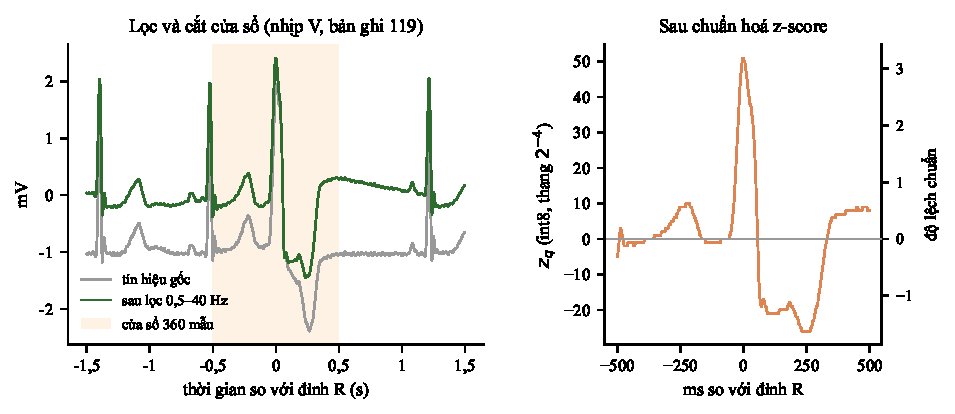
\includegraphics[width=\textwidth]{ch04_mo_hinh_cnn/mot_nhip.pdf}
  \caption{Một nhịp V của bản ghi 119: tín hiệu trước và sau bộ lọc 0{,}5--40\,Hz với vùng cửa sổ 360 mẫu (trái), và cửa sổ sau chuẩn hoá z-score số nguyên (phải).}\label{fig:ch4-motnhip}
\end{figure}

\subsection{Đặc trưng khoảng RR}

Nhịp S chủ yếu khác nhịp N ở thời điểm xuất hiện, thông tin mà cửa sổ một nhịp không có, nên mạng nhận thêm bốn đặc trưng nhịp điệu.
Với $\mathrm{RR}_k=R_k-R_{k-1}$, kẹp trong 0{,}2--3\,s để loại giá trị phi sinh lý:
\begin{equation}
  \mathrm{RR}_{\text{trước}}=\mathrm{RR}_k,\qquad
  \mathrm{RR}_{\text{sau}}=\mathrm{RR}_{k+1},\qquad
  \overline{\mathrm{RR}}=\frac{1}{n}\sum_{j=0}^{n-1}\mathrm{RR}_{k-j},\qquad
  \rho=\frac{\mathrm{RR}_{\text{trước}}}{\overline{\mathrm{RR}}},
  \label{eq:ch4-rr}
\end{equation}
với $n\le8$.
Tỉ số $\rho$ tự chuẩn hoá theo nhịp tim của từng người: nhịp đến sớm có $\rho<1$ dù nhịp tim nhanh hay chậm.
Các đặc trưng chỉ cần thêm một khoảng RR kế tiếp, nên mỗi nhịp chỉ chờ đến đỉnh R sau nó.

\begin{table}[htbp]
  \centering
  \caption{Trung vị của đặc trưng RR theo lớp trên DS1.}\label{tab:ch4-rr}
  \begin{tabular}{lrrrr}
    \toprule
    Đặc trưng & N & S & V & F \\
    \midrule
    $\mathrm{RR}_{\text{trước}}$ (s) & 0{,}756 & 0{,}492 & 0{,}522 & 0{,}592 \\
    $\mathrm{RR}_{\text{sau}}$ (s) & 0{,}736 & 0{,}644 & 0{,}856 & 0{,}461 \\
    $\rho$ & 1{,}00 & 0{,}83 & 0{,}74 & 0{,}96 \\
    \bottomrule
  \end{tabular}
\end{table}

Theo Bảng~\ref{tab:ch4-rr}, nhịp S và V đến sớm ($\rho$ khoảng 0{,}83 và 0{,}74), và nhịp V có khoảng nghỉ bù dài phía sau.
Nhịp F có $\rho$ gần 1, gần như không khác nhịp N về thời điểm, nên chỉ phân biệt được bằng hình dạng; đây là một lý do lớp F khó nhận diện nhất.

Mỗi đặc trưng được lượng tử về int8 với thang $2^{-e_j}$, $e_j=(6,6,6,5)$, bằng một phép chia làm tròn, ví dụ $\mathrm{rr}_{q,0}=\lfloor\mathrm{RR}_{\text{trước}}\cdot2^{6}/360\rceil$; tỉ số được tính thẳng từ tổng các khoảng RR để chỉ chia một lần.
Như vậy khoảng RR có độ phân giải $1/64$\,s, tối đa khoảng 1{,}98\,s, còn tỉ số tối đa khoảng 3{,}97.

% Muc 4.3  --  phu trach: xem report/PHANCONG.md
\section{Kiến trúc CNN Lite}\label{sec:cnnlite}
\begin{goiy}
  \begin{itemize}
    \item Bốn block Conv(k=7,5,3,3) + BN + ReLU + MaxPool, GAP, FC1 $68\to32$, FC2 $32\to4$ (Bảng~\ref{tab:cnnlite}).
    \item Số liệu: 23\,408 B trọng số int8 + 212 bias int32; 1\,609\,344 MAC/nhịp; trường nhìn $\approx128$~ms.
    \item Minh hoạ một nhịp qua các tầng (Hình~\ref{fig:trace}).
  \end{itemize}
\end{goiy}
\bangcho{từng lớp: vào$\to$ra, kernel, số tham số, MAC/nhịp (xem docs/cnn\_explained.md §1)}{Kiến trúc CNN Lite và chi phí tính toán mỗi lớp.}{tab:cnnlite}

\begin{figure}[htbp]
  \centering
  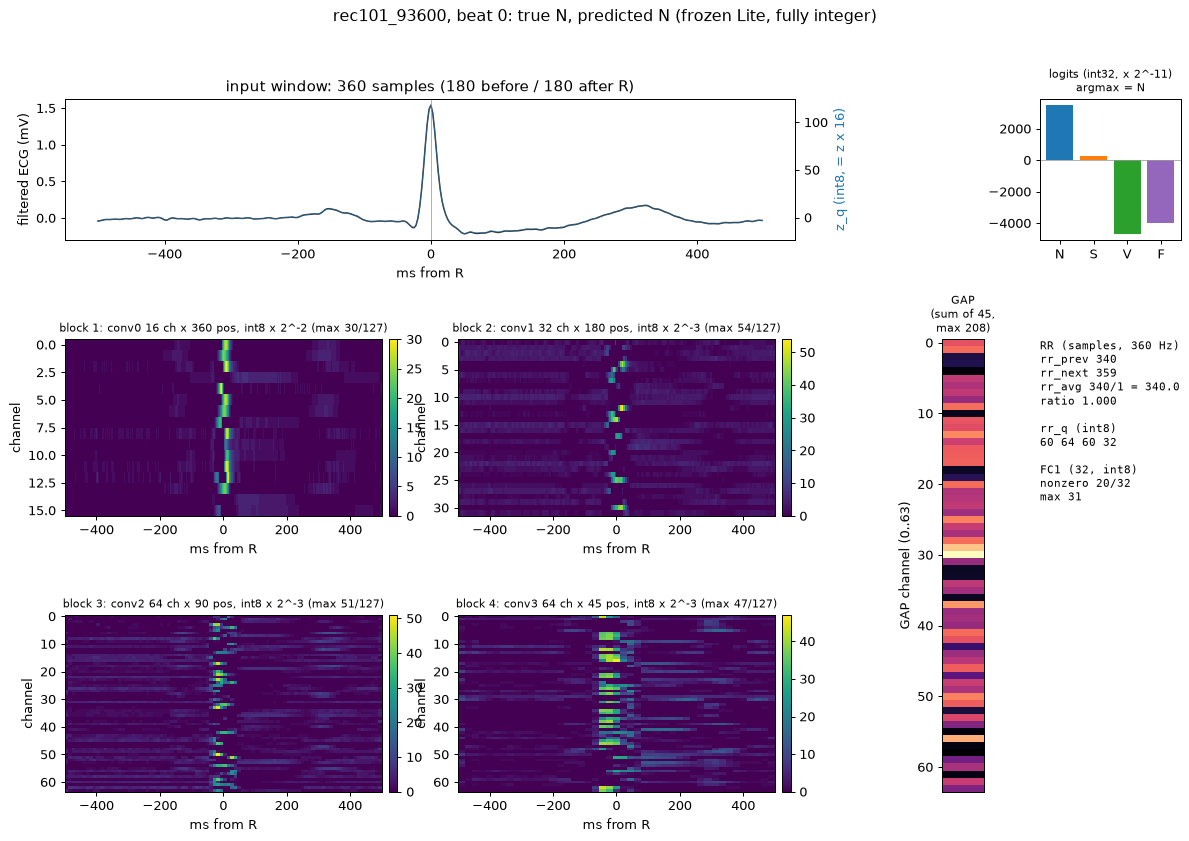
\includegraphics[width=\textwidth]{ch04_mo_hinh_cnn/trace_rec101_beat0.png}
  \caption{Một nhịp N (rec101) qua pipeline số nguyên: cửa sổ vào, feature map 4 block và logit.}\label{fig:trace}
\end{figure}

% Muc 4.4  --  phu trach: xem report/PHANCONG.md
\section{Huấn luyện}\label{sec:huanluyen}
\begin{goiy}
  \begin{itemize}
    \item Focal loss ($\gamma=2$) + trọng số lớp sqrt-inverse; AdamW (lr $10^{-3}$, wd $10^{-2}$), 3 epoch; thêm SVDB (n25) chỉ trong inner-train.
    \item Các lựa chọn đã thử (ablation) và vì sao chọn Lite thay vì Full.
    \item Mô hình đóng băng (SHA-256 trong \texttt{export/final\_models\_manifest.json}).
  \end{itemize}
\end{goiy}

% Muc 4.5  --  phu trach: xem report/PHANCONG.md
\section{Lượng tử hoá int8}\label{sec:luongtu}
\begin{goiy}
  \begin{itemize}
    \item Gộp BN vào conv $W'=W\gamma/\sqrt{\sigma^2+\epsilon}$; gộp 1/45 của GAP và z-score RR vào FC1.
    \item Scale luỹ thừa 2; trọng số theo kênh; requantize $y=\mathrm{clamp}\big((acc+2^{s-1})\gg s,0,127\big)$; ReLU = kẹp.
    \item Logit int32 cùng scale $2^{-11}$; argmax thay softmax (chứng minh đơn điệu).
    \item Ngân sách int32 (kiểm tràn) và sai khác so với float (cổng lượng tử).
  \end{itemize}
\end{goiy}

% Muc 4.6  --  phu trach: Hùng
% nguon: export/golden_manifest.json cua repo 1DCNN (8 doan, 1 306 phat hien, nhan: 649 N, 307 S, 295 V, 51 F, 1 Q, 3 khong khop)
\section{Bộ dữ liệu chuẩn}\label{sec:golden}

Bộ dữ liệu chuẩn, gọi là golden vectors, ghi lại đầu ra của từng tầng trong pipeline số nguyên khi xử lý một số đoạn tín hiệu cố định.
Nó đóng vai trò đáp án cho mọi cài đặt lại của pipeline: mô phỏng RTL hay bộ tăng tốc trên board đều phải cho kết quả khớp từng bit với bộ dữ liệu này.

\subsection{Thành phần}

Bộ dữ liệu gồm tám đoạn tín hiệu dài 120\,s, lấy từ tám bản ghi khác nhau của DS1.
Ở mỗi bản ghi, đoạn được chọn là đoạn chứa nhiều nhịp bất thường nhất, để bộ dữ liệu bao phủ đủ bốn lớp thay vì chủ yếu là nhịp N như dữ liệu gốc.
Trên tám đoạn, bộ phát hiện tìm được 1\,306 nhịp; trong đó 1\,302 nhịp khớp với nhãn gồm 649 nhịp N, 307 nhịp S, 295 nhịp V và 51 nhịp F, bốn nhịp còn lại là nhịp lớp Q hoặc phát hiện không khớp nhãn nào.
Các phát hiện không khớp vẫn được giữ lại, vì phần cứng xử lý mọi nhịp mà bộ phát hiện đưa ra chứ không biết trước nhãn.
Mỗi đoạn được xử lý từ trạng thái ban đầu bằng không, giống như hệ thống vừa khởi động.

Với mỗi nhịp, bộ dữ liệu lưu:
\begin{itemize}
  \item đầu vào của mạng: cửa sổ $z_q$ và bốn đặc trưng $\mathrm{rr}_q$;
  \item đầu ra của từng lớp tích chập và từng lớp gộp cực đại;
  \item tổng của phép lấy trung bình toàn cục và đầu ra lớp FC1;
  \item bốn logit int32 và nhãn dự đoán.
\end{itemize}
Ngoài ra, các tín hiệu trung gian của khối tiền xử lý theo từng mẫu cũng được lưu, cùng với toàn bộ trọng số, bias và lượng dịch để nạp cho phần cứng.

\subsection{Vai trò trong kiểm chứng}

Nhờ lưu đủ các tầng trung gian, khi phần cứng cho kết quả sai có thể xác định ngay lớp đầu tiên bị lệch thay vì chỉ biết nhãn cuối cùng sai.
Điều này cho phép kiểm chứng bộ tăng tốc theo từng lớp trong quá trình phát triển, trước khi chạy trọn mạng; quy trình và kết quả kiểm chứng được trình bày ở Mục~\ref{sec:bitexact}.

Cần lưu ý rằng các đoạn này thuộc DS1, tức dữ liệu mô hình đã thấy khi huấn luyện.
Vì vậy bộ dữ liệu chuẩn chỉ dùng để kiểm chứng tính đúng của cài đặt, không dùng để đánh giá khả năng tổng quát hoá; khả năng này chỉ được đánh giá trên DS2.

